\DAsection[读标记、解冲突、保护 main]{冲突处理、Review 与主分支治理}

\begin{frame}[fragile]{4.1 先学会读冲突标记}{当前分支、分隔线、待合并分支}
  \centering
  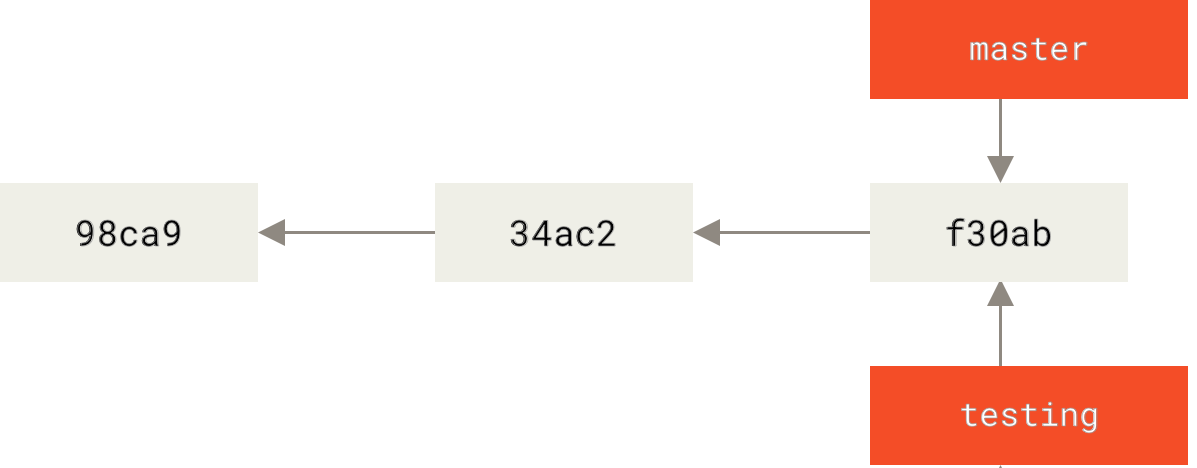
\includegraphics[width=48mm]{assets/official/collected/git-two-branches.png}
  \begin{lstlisting}
<<<<<<< HEAD
const apiBase = "/api";
=======
const apiBase = "http://localhost:8000";
>>>>>>> feature/api-config
  \end{lstlisting}
  \begin{itemize}
    \item 先确认生产架构与配置约定，再选择或融合两侧代码。
    \item 删除全部标记后，必须重新运行测试与构建。
  \end{itemize}
  \DAsource{Pro Git · Divergent Branches}{https://git-scm.com/book/en/v2/Git-Branching-Branches-in-a-Nutshell}
\end{frame}

\begin{frame}[fragile]{4.2 命令行解决冲突的标准步骤}{定位、编辑、验证、继续}
  \begin{lstlisting}[language=bash]
git status
# open conflicted files and resolve markers

pnpm lint
pnpm test
pnpm build

git add src/config/api.ts
git commit                 # merge workflow
# or: git rebase --continue
  \end{lstlisting}
  \begin{itemize}
    \item \DAcmd{git status} 会列出所有未合并路径。
    \item 不确定时可用 \DAcmd{git merge --abort} 或 \DAcmd{git rebase --abort} 回到操作前。
    \item 解决冲突时必须理解两边业务意图。
  \end{itemize}
\end{frame}

\begin{frame}{4.3 GitHub 在线解决简单行冲突}{复杂冲突回到本地测试}
  \centering
  \DAframed{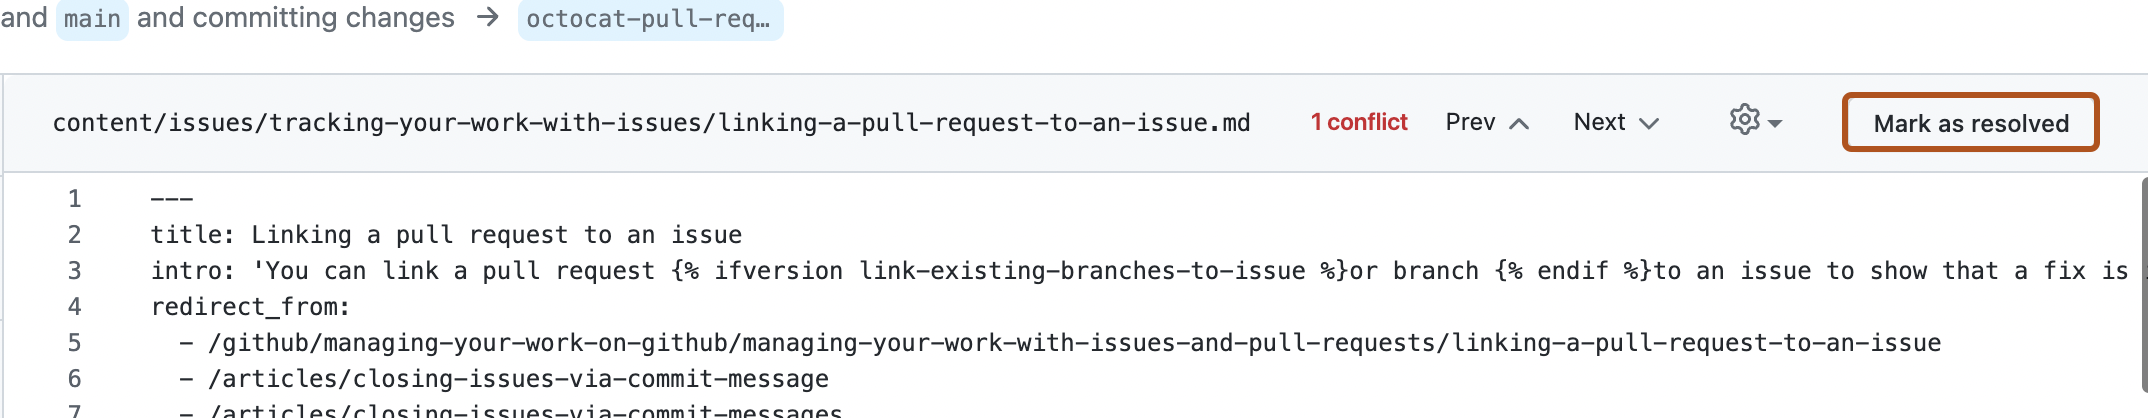
\includegraphics[width=119mm]{assets/official/github-conflict-editor.png}}
  \begin{itemize}
    \item 简单的竞争行可以使用网页冲突编辑器。
    \item 删除 / 重命名、生成文件、依赖锁文件等复杂冲突建议本地处理。
    \item 合并前必须验证构建、测试和关键业务流程。
  \end{itemize}
  \DAsource{GitHub Docs · Resolving a merge conflict}{https://docs.github.com/en/pull-requests/collaborating-with-pull-requests/addressing-merge-conflicts/resolving-a-merge-conflict-on-github}
\end{frame}

\begin{frame}{4.4 如何减少冲突}{重点是工作拆分、同步和接口约定}
  \begin{columns}[T]
    \begin{column}{0.54\textwidth}
      \begin{itemize}
        \item 拆成小任务，使用短生命周期分支。
        \item 明确模块负责人，减少同时修改核心文件。
        \item 频繁同步 \DAfile{main}，尽早暴露竞争变化。
        \item Schema、路由和公共配置先约定再编码。
        \item 格式化与依赖更新单独提交。
      \end{itemize}
    \end{column}
    \begin{column}{0.42\textwidth}
      \centering
      \DAframed{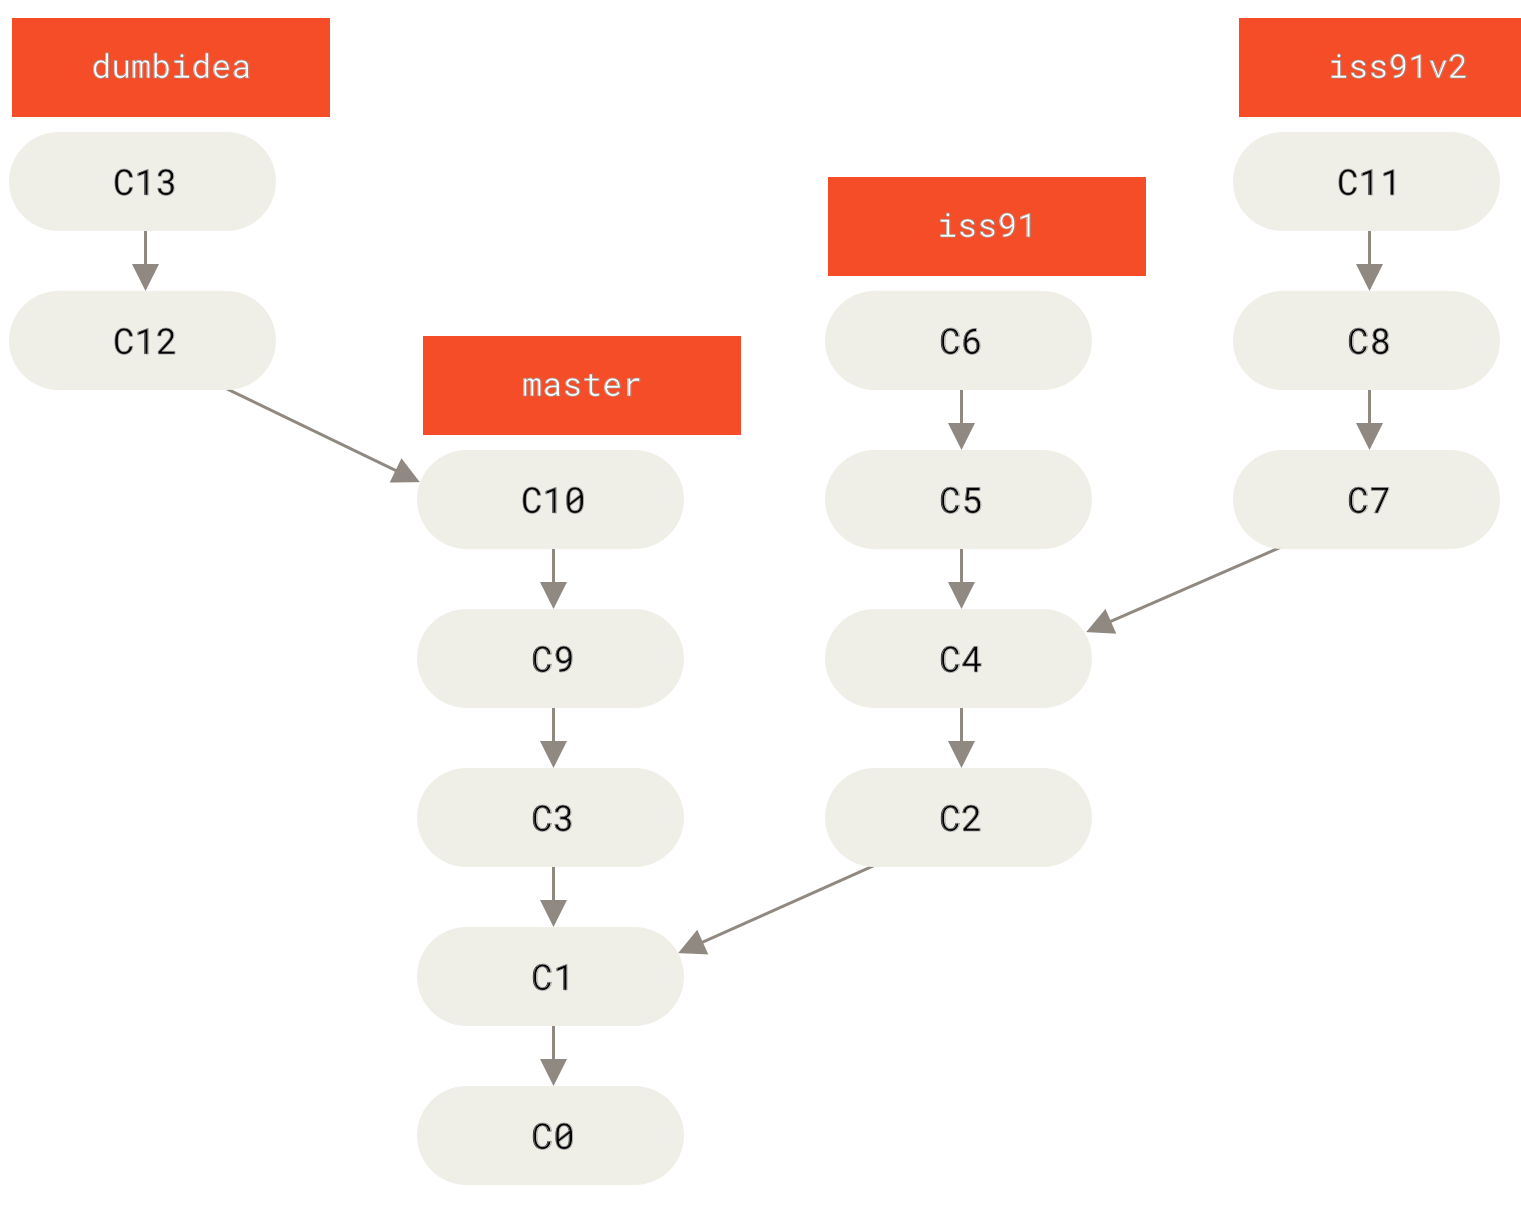
\includegraphics[width=46mm]{assets/official/collected/git-topic-branches.png}}
      \par\smallskip
      {\scriptsize 一个分支只承载一个清晰任务。}
    \end{column}
  \end{columns}
  \DAsource{Pro Git · Topic Branches}{https://git-scm.com/book/en/v2/Git-Branching-Branching-Workflows}
\end{frame}

\begin{frame}{4.5 Rebase 为什么需要谨慎}{它会把 Commit 复制到新的父节点上}
  \centering
  \DAframed{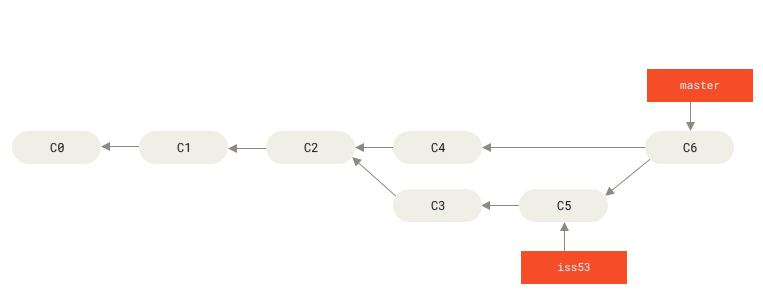
\includegraphics[width=84mm]{assets/official/collected/git-basic-merge.png}}
  \begin{itemize}
    \item Merge 保留分叉历史；Rebase 会复制提交到新的父节点。
    \item Rebase 后 Commit ID 改变，远程推送可能需要历史重写。
    \item 只重写自己的功能分支；共享历史保持稳定。
  \end{itemize}
  \DAsource{Pro Git · Basic Merging}{https://git-scm.com/book/en/v2/Git-Branching-Basic-Branching-and-Merging}
\end{frame}

\begin{frame}[fragile]{4.6 Rebase 后推送用 force-with-lease}{它会检查远程分支是否被别人更新}
  \begin{lstlisting}[language=bash]
git fetch origin
git rebase origin/main

git push --force-with-lease
  \end{lstlisting}
  \begin{alertblock}{禁止使用}
    \DAcmd{git push --force} 可能覆盖同事刚推送的 Commit。
  \end{alertblock}
  \DAtagline{边界}{如果团队尚未理解历史重写，统一用 Merge 同步 main 更安全}
\end{frame}

\begin{frame}{4.7 主分支保护规则}{main 始终代表“可部署版本”}
  \begin{itemize}
    \item 禁止直接 Push，所有变化通过受控合并流程进入 \DAfile{main}。
    \item 至少一人 Approve，关键目录可配置 CODEOWNERS。
    \item 必须通过构建、测试、Lint 等状态检查。
    \item 必须解决 Review 对话后才能合并。
    \item 默认禁止 Force Push 与删除主分支。
  \end{itemize}
  \DAtagline{结果}{规则把“团队口头约定”变成平台自动执行的门禁}
  \DAsource{GitHub Docs · About protected branches}{https://docs.github.com/en/repositories/configuring-branches-and-merges-in-your-repository/managing-protected-branches/about-protected-branches}
\end{frame}
